\documentclass{beamer}
\usepackage{bbm}
\usepackage{graphicx,wrapfig,lipsum}

%Information to be included in the title page:
\title{Optimization with large learning rate}
% \author{Denis Grachev} 

\author[author1]{Denis Grachev\\[10mm]{\small supervisor: Yurii Malitsky}}


\institute{University of Vienna}

\date{\today}

\begin{document}

\frame{\titlepage}
\graphicspath{{./images/}}

\begin{frame}
\frametitle{Defenitions}

$$ f_* := \min_{x \in \mathbb{R}^d} f(x)$$
$f$ is $L$-smooth and 
$\mu$-one-point-strongly-convexity (OPSC) with respect to $x_\ast$ over $M \subset \mathbb{R}^d$.

\begin{definition}[$f: \mathbb{R}^d \rightarrow \mathbb{R}$ is $L$-smoothness]
	\begin{itemize}
		\item $f$ is differentiable.
		\item $\exists L: \| \nabla f(x) - \nabla f(y)\| \leq L \| x - y \|$ .
	\end{itemize}
\end{definition}

\begin{definition}[ $f: \mathbb{R}^d \rightarrow \mathbb{R}$ is $\mu$-one-point-strongly-convex (OPSC) with respect to $x_\ast$ over $M$]
	\begin{itemize}
		\item $f$ is differentiable
		\item $\exists \mu > 0: \langle \nabla f(x), x - x_\ast \rangle \geq \mu \| x - x_\ast\|^2, \: \forall x \in M$.
	\end{itemize}
  
\end{definition}

\end{frame}

\begin{frame}{Motivation}
	\begin{itemize}
		\item Standart threshold for learning rate in Gradient Descent is $\gamma < \frac{2}{L}$.
		\item For neural networks it has been widely observed that larger lerarning rates often obtain better models.
		\item In the  \href{https://arxiv.org/pdf/2205.15142.pdf}{\color{blue}article} new theorems are presented about usage of larger learning rates in GD. 
		\item Show the theorems and present performed experiments.
	\end{itemize}
\end{frame}


\begin{frame}{Lemma 1}

\begin{itemize}
	\item $f$ is $L_{\text{global}}$-smooth.
	\item $f$ has global minima $x_\ast$ and local $x^\dagger$.
	\item $f$ is $\mu^{\dagger}$-OPSC with respect to  $x^\dagger$ over a set $M$ with diameter $r$.
	\item $P(M) = B_{r_P}(x^\dagger) \setminus M$. 
	\item $f$ is $L < L_{\mathrm{global}}$ -smooth in $P(M)$ and $\mu_\ast$-OPSC with respect to $x_\ast$ and $\mu^\dagger > \frac{2L^2}{\mu_\ast}$.
	\item $x^\dagger$ is sufficiently far from $x_\star$.

\end{itemize}
Then using GD with $\frac{2}{\mu^{\dagger}} < \gamma < \frac{\mu_\ast}{L^2}$ if reach $M$
GD will escape $M$ and reach a point closer to $x_\ast$ than 
$\| x^\dagger - x_\ast\| - r$ almost surely.
	\begin{figure}[h]
	%\begin{wrapfigure}{r}{0.5\textwidth}
	     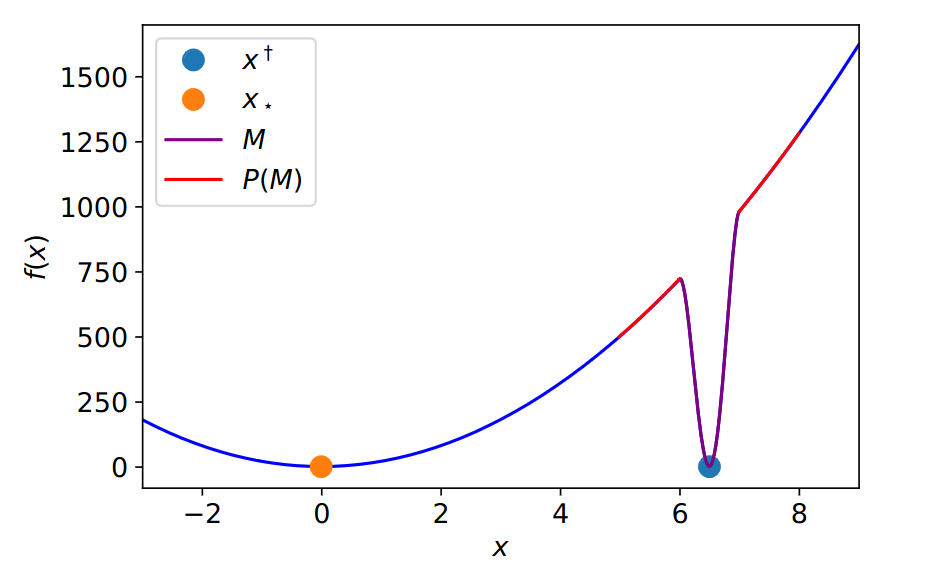
\includegraphics[scale=0.2]{lemma1}
	\end{figure}
	%\end{wrapfigure}

\end{frame}


\begin{frame}
\frametitle{Theorem 1}
\begin{itemize}
	\item $f$ is $L$-smooth.
	\item $f$ is $\mu_\ast$-OPSC with respect to the 
	 global minima $x_\ast$ except the region $M$ that 
	 contains local minima $x^\dagger$.
	\item $x^\dagger$ satisfies Lemma 1.
\end{itemize}
Then
\begin{itemize}
	\item $\gamma < \frac{\mu^{\dagger}}{L^2_{\text{global}}}$\\
	GD initialized randomly inside $M$ converges to $x^\dagger$.
	\item $\frac{2}{\mu^{\dagger}} < \gamma \leq \frac{\mu_\ast}{L^2}$ \\
	GD initialized randomly inside $W: \mathcal{L}(W) > 0$ 
	will converge to $x^\ast$ almost surely.
\end{itemize}

\end{frame}

\begin{frame}
\frametitle{Lemma 2}
\begin{itemize}
	\item GD initialized randomly in $W$ with $\gamma \leq \frac{1}{2L}$
	\item $X \subset \mathbb{R}^d$ arbitrary set of points in the landscape, $f$ is $L$-smooth over $\mathbb{R}^d \setminus X$
\end{itemize}

Then probabilty of encountering 
 any point of $X$ in first $T$ steps is 
 at most $2 ^ {(T + 1)d} \frac{\mathcal{L}(X)}{\mathcal{L}(W)}$
\end{frame}

\begin{frame}
\frametitle{Theorem 2}
\begin{itemize}
	\item $X$ be an arbitrary set of points.
	\item $f$ is $\mu_\ast$-OPSC with respect to a minima 
	$x_\ast \notin X$ over $\mathbb{R}^d \setminus X$.
	\item $c_X := \inf \left\{ \| x - x_\ast \| \:|\: x \in X  \right\}$
	\item $r_W := \sup \left\{ \| x - x_\ast \| \:|\: x \in W \right\}$
	
\end{itemize}
Then probability of not encountering any points of $X$ during 
gradient descent with learning rate $\gamma \leq \frac{\mu_\ast}{L^2}$ is at least

\begin{itemize}
	\item $c_X \leq r_W$ \\
	$1 - \frac{r_W}{c_X}^{\frac{-d}{\log_2(1 - \gamma \mu_\ast)}} \frac{\mathcal{L}(X)}{\mathcal{L}(W)} 2^d$
	\item otherwise \\
	1
\end{itemize}

\end{frame}



\begin{frame}{Example 1D}
    $$
    f(x):= \begin{cases}        
        % \left(
            -1600(x-2.5)^5-2000(x-2.5)^4 + \\
            \quad +800(x-2.5)^3+1020(x-2.5)^2
        % \right) 
        & 2 \leq x \leq 3 \\ 
        1411.2 \times\left(1-10^4(x-8.4)\right) & 8.4 \leq x \leq 8.40001 \\ 
        0 & 8.40001 \leq x \leq 8.59999 \\ 
        1479.2 \times\left(10^4(x-8.6)+1\right) & 8.59999 \leq x \leq 8.6 \\ 
        20 x^2 & \textit{ otherwise }
    \end{cases}
    $$
    
    \begin{itemize}
    	\item Run GD with different start point and learning rate. \\
    	$x_{\text{start}} \in \text{linespace}(8.5, 10, 20)$ \\
    	$lr \in \text{logspace}(-4, -0.5, 25)$
    	\item Plot obtained minima and trajectories.
    	\item Demo.
    \end{itemize}
    

\end{frame}

\begin{frame}{Example 2D}
	\begin{align*}
		f(x, y) := 
			&x^2 + y^2 - \\
			&200 \mathrm{ReLU}(|x|-1) \mathrm{ReLU}(|y|-1) \\
			&\mathrm{ReLU}(2-|x|) \mathrm{ReLU}(2-|y|)
	\end{align*}
	
	\begin{itemize}
		\item Run GD with different start point and learning rate.\\
		$x_{\text{start}}$ random in $\left[3, 4\right] \times \left[3, 4\right]$. 30 samples. \\
		$lr \in \text{logspace}(-1.75, -1.6, 25)$
		\item Plot trajectories.
		\item For each learning rate calculate share of each minima.
		\item Demo.
	\end{itemize}
	 	
\end{frame}
    
\begin{frame}{Brief introduction to ML}
	\begin{itemize}
		\item Dataset\\
		 $D := \{(x_1, y_1), (x_2, y_2) \ldots (x_n, y_n) \:\|\: x_i \in \mathbb{R}^k, y_i \in C \}$
		 \item NN with p parameters\\
		 $f: \mathbb{R}^k \times \mathbb{R}^p \rightarrow \mathbb{R}^t$\\
		 \item Loss function\\
		 $\mathcal{L}: \mathbb{R}^t \times C \rightarrow \mathbb{R} $
		 \item Total Loss\\
		 $\mathcal{L}_{\text{total}}(D, \theta) = \sum_{i=1}^{n} l(f(x_i, \theta), y_i)$
		 \item Training\\
		 $\min_{\theta \in \mathbb{R}^p} \mathcal{L}(D, \theta)$
		 \item Overfitting\\
		 Dataset is splitted into training and testing
	\end{itemize}

\end{frame}

\begin{frame}{Dataset}

\begin{itemize}
	\item Mnist dataset.
	\item Pictures $28 \times 28$ pixels of numbers.
	\item 60000 training and 10000 validation sizes.
	\item $C = \{0, 1, 2, \ldots, 9 \}$, $t = 10$
\end{itemize}

\begin{figure}[h]
    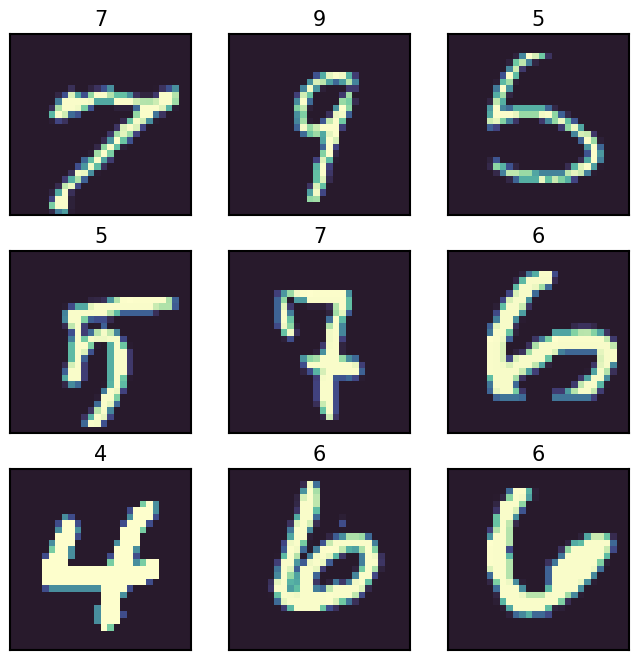
\includegraphics[scale=0.3]{mnist}
\end{figure}

\end{frame}

\begin{frame}{Loss function}
	Cross entropy loss.
    
    $\mathcal{L}: \mathbb{R}^t \times C \rightarrow \mathbb{R}$ \\
    $\mathcal{L}(\hat{y}, y) := -\sum_{i=1}^c \mathbbm{1}_{i == y} \log\left(\frac{\exp{y_i}}{\sum_{j=1}^c \exp{y_j}}\right) = -\log(p_{\text{true}})$ \\
    
    \begin{figure}[h]
    	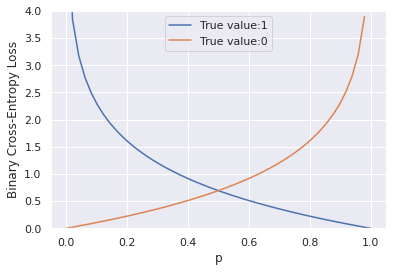
\includegraphics[scale=0.5]{binary-cross-entropy-loss}
    \end{figure}

\end{frame}


\begin{frame}{Structure of NN}
    Structure of NN is 
    $$f = f_k \circ \mathrm{Linear}_k \circ \ldots \circ f_1 \circ \mathrm{Linear}_1$$
    where $\mathrm{Linear}_i$ is some linear function and $f_i$ is a non linear elementwise function.

    For $f_i$ taken $\mathrm{ReLU}$
    $$ 
    \mathrm{ReLU}(x) := \begin{cases}
    x & x > 0 \\
    0 & x \leq 0
    \end{cases} 
    $$
    
    Total test structure
    $$ f = \mathrm{ReLU} \circ \mathrm{Linear}(16, 10) \circ \mathrm{ReLU} \circ \mathrm{Linear}(32, 16) \circ \mathrm{ReLU} \circ \mathrm{Linear}(784, 32)$$

\end{frame}

\begin{frame}{Analyzis of NN}
	\begin{itemize}
		\item 3 initial position were taken.
		\item From each position 3 GD with different learning rates started.
		\item Parameters were reduced to 2 dimensional space using PCA.
		\item Trajectories ploted.
	\end{itemize}
	
	\begin{figure}
	\caption{PCA example}
	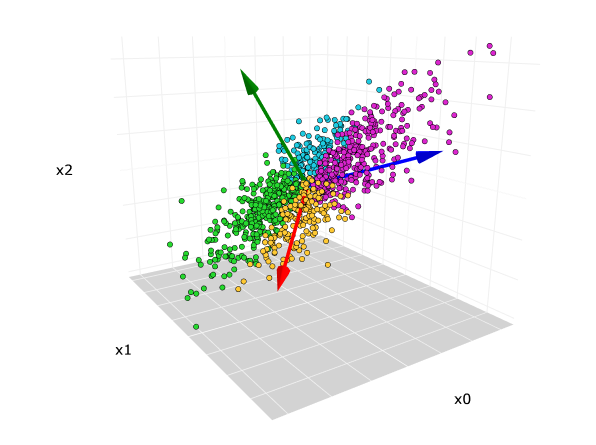
\includegraphics[scale=0.3]{pca}
	\end{figure}
\end{frame}

\begin{frame}{End}
	  \centering \Large
	  \emph{Thank you for your attention!}
\end{frame}

\end{document}